%=================================================================
\documentclass[dvipdfmx]{issj}
%=================================================================
% 情報システム学会 研究発表大会 原稿用テンプレートの利用例
%     ISSJ実行委員会/プログラム委員会(ISSJ学会誌編集委員会)
% issj2012.sty Ver. 0.50 2012-10-12 Tadashi Iijima (iijima@ae.keio.ac.jp)
% issj2012.sty Ver. 0.60 2012-10-15 Tadashi Iijima (iijima@ae.keio.ac.jp)
% issj2012.sty Ver. 0.70 2012-10-19 Tadashi Iijima (iijima@ae.keio.ac.jp)
% issj2012.sty Ver. 0.80 2012-10-20 Tadashi Iijima (iijima@ae.keio.ac.jp)
%=================================================================
\title{「Twitter上で共感を生み出すツイートの性質に関する考察」の検証}
%-----------------------------------------------------------------
\etitle{Verification of "Consideration on Characteristics of Sympathy-arousing Tweets on Twitter"}
%-----------------------------------------------------------------
\author{木村 咲\uddag, 松澤芳昭\uddag}
%-----------------------------------------------------------------
\eauthor{Saki Kimura\udag, and Yoshiki Matsuzawa\uddag}
%-----------------------------------------------------------------
\affiliation{\dag 青山学院大学 社会情報情報学部\ddag }
%-----------------------------------------------------------------
\eaffiliation{\dag School of Social Informatics, Aoyama Gakuin University.}
%-----------------------------------------------------------------
%=================================================================
\begin{document}
%=================================================================
\maketitle
%=================================================================
\begin{abstract}
本研究では、先行研究で実証されていた「Twitter上で共感を生み出すツイートの性質」の再現性を確認するための追試を行った。 追試では先行研究とは異なるツイートデータを対象とし、新たに属性として「画像の有無」と「感情極性値」を追加した。 芸能人4名のデータを収集して分析した結果、全ての属性においてTwitterで共感を生み出す性質は見られなかった。 これは先行研究と(A)ツイートの時期、(B)ラベル付けした被験者が異なるためだと考えられる。
\end{abstract}
%=================================================================
\section{はじめに} %%%% 第1節
%=================================================================

近年はSNS上で買い物ができるようになったり、またYoutuberやインスタグラマーなどSNSを利用して稼ぐ人も増え、今後よりSNSのマーケティングは盛んになるだろう。
中でもSNSを運用するにあたって共感の注目が高まっており、日本企業の約63.9%がSNS運用でユーザーの共感の獲得が目標の指標になっている。[A] 
またSNSで注目されている共感だが、共感については動物行動学、教育心理学、社会心理学、臨床心理学や脳神経生理学など他分野で多面的、学際的にアプローチされ、研究が行われており、その時々で共感の定義そのものも、多様であり、捉え方も様々である。[B]
そこで本稿では、Twitterで共感を生み出すツイートはどのような性質があるのかを調査する。





%========================================================================
\section{先行研究と本研究の目的}  %%%% 第2節
%========================================================================

共感は、従来さまざまな観点から多くの分野で研究されてきた。
大川, 高間の研究[1]では、不特定の相手向けになされたツイート(つぶやき)に対し多数の人が共感を抱くケースに着目し、その発生のメカニズムの解明を行った。
不特定多数のユーザーが閲覧するツイートを対象とするため、ここでは著名人のツイートデータを対象としている。
第一著者の判断により共感が発生しているか否かのラベル付けを行うと同時に、それらのツイートの「いいね数」や「RT数」「文字数」など計11個の属性(表1)の値も取得した。
その結果、「文字数が少ないツイート」と「悲しみを含むツイート」が共感を生み出しやすいことが判明した。
文字数が影響を及ぼしてる理由としては、ツイートの長さが冗長であればあるほどユーザーがテキストの全てを閲覧することがなくなり、共感の発生を妨げる原因になってる可能性があるからだ。
また悲しみを含むツイートは、人間は悲しい記憶が残りやすく、そのためツイートを投稿したユーザーの状況をイメージしやすくなり、共感が発生する可能性が高くなるためだと考察していた。
そこで本研究では、この結果は別のツイートでも再現可能なのかを検証するため、ツイート内容を変えて追試を行った。
加えて本稿ではImage(画像の有無)という新たな属性も加えた。
これは、ツイートに画像が添付されることによってツイート内容のイメージを湧きやすくさせる効果があり、共感にも影響を及ぼすと考えるからだ。



\begin{table}[h]\centering
\caption{属性名と属性値の形式}\label{tbl:font}
\begin{small}
\begin{tabular}{|c|c|} \hline
属性名            & 属性値の形式\\\hline\hline
fav & real 型, 0~\\\hline
rt  &  real 型, 0~\\\hline
term  & real 型, 0~\\\hline
characters         & real 型, 0~\\\hline
unofficial      &  real 型, 1~140\\\hline
gladness & {yes, no}\\\hline
anger & {yes, no}\\\hline
sadness & {yes, no}\\\hline
pleasure & {yes, no}\\\hline
sadness & {yes, no}\\\hline
agreement & {agree, disagree, neutral}\\\hline
thinking & {positive, negative, neutral}\\\hline
\end{tabular}
\end{small}
\end{table}



%========================================================================
\section{共感の定義}  %%%% 第3節
%========================================================================

先行研究ではTwitter上におけるツイートに対する共感を「そのツイートを不特定多数のユー ザが閲覧したときに,投稿した背景が想像でき,そ れに同感できる」ことであると定義している。
つまり、ツイートに同感できないと共感は成り立たないことを意味している。
しかし、佐伯は「同感」と「共感」を別物と捉える。
「同感というのはその人の感じていることと自分の感じていることを同じなのだと思うこと」であり,そこには未知なる世界への探求も,新しい発見もなく,「相手は自分と同じだという確認」があるに過ぎない。
一方の共感とは,「白分にはすてきとは思えないが,その良さをわかりたい」というように,「その人が良いといっているのはどういうところなのだろうということを探求して「理解」しようとする。そこにいたる経緯やそこでの状況をしっかり把握して,その場に我が身をおいて,なんとかして,そこでの「良さ」を,心底「納得」しようとする」ことと捉えられている。18).
またロジャーズによると、共感とは「自分が自分が他者であるかのような、しかし”かのようにas if”という状態を失わずに関係する。正確さや感情的要素、意味を持って他者の内部関連気分を知覚すること」と唱えられいてる。
この2つをもとに本研究では共感を、「不特定多数のユーザーがそのツイートを閲覧したとき、投稿した背景が想像でき、そのツイート(投稿者)の内部関連気分を汲み取れること」と定義する。
ゆえに、以下の2項目が成り立つとき、そのツイートは共感できるツイートとする。

\begin{table}[h]\centering
\caption{共感できるかの判断基準}\label{tbl:font}
\begin{small}
\begin{tabular}{|c|c|} \hline
項目   & 詳細\\\hline\hline
1& ツイートの背景が記載されているツイート\\\hline
2 & 投稿者の感情が汲み取れるツイート\\\hline
\end{tabular}
\end{small}
\end{table}


%------------------------------------------------------------------------
\subsection{ツイートの収集と共感のラベル付け }  %%%% 第3.1節
%------------------------------------------------------------------------
今回は芸能人の中でもフォロワー数が最も多い芸能人男女4名を分析対象とし、2021年7月27日から最新のツイートデータをそれぞれ50件収集した。
使用するデータは、第一次情報源でない「公式リツイート」と、特定の相手を対象としたつぶやきである「リプライ」は除いている。
TwitterAPIを用いてツイートを取得し、取得したツイートに対して共感したか否かを手作業によってラベル付けを行った。
共感を生み出すとラベル付けされたツイートと、共感を生み出さないとラベル付けされたツイートの例を画像1と画像2に示す。
まず、画像1は共感を生み出すと判断されたツイートだ。
これは、吉高由里子が”自分の誕生日に周りに祝ってもらって嬉しくてツイートした”という背景と、”祝ってもらって嬉しい”という感情が伺える。
これは、図1の2つの条件を満たしているため共感できるツイートだとラベル付けした。
続いて、画像2は共感を生み出さないと判断されたツイートだ。
このツイートからは、吉高由里子が”誰かと手持ち花火をしている”というツイートの背景が確認できる。
しかし、感情面については言及されていないため判断することができない。
つまり、図1の1つの条件を満たしていないため共感を生み出さないツイートとラベル付けした。

\begin{figure}[htbp]
 \begin{minipage}{0.5\hsize}
  \begin{center}
 
\includegraphics[width=80mm]{fig1.png}
  \end{center}
\caption{共感を生み出すツイート}  \label{fig:one}
 \end{minipage}

 \begin{minipage}{0.5\hsize}
  \begin{center}
 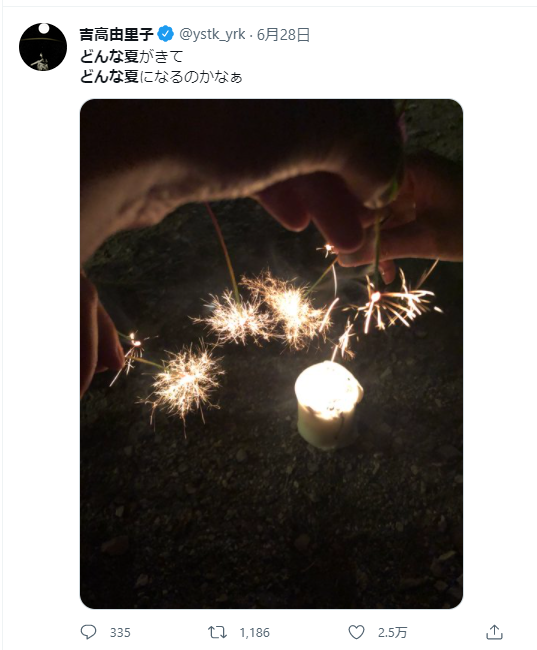
\includegraphics[width=80mm]{fig2.png}
  \end{center}
\caption{共感を生み出さないツイート}  \label{fig:two}
 \end{minipage}
\end{figure}





%------------------------------------------------------------------------
\subsection{属性の定義と抽出方法}  %%%% 第3.2節
%------------------------------------------------------------------------
本稿で用いる属性を表◯に示す。
これらの属性は先行研究の属性に加え、~~~を加えたものである。
先行研究では、共感に関係すると考えられるもののうち、Twitter 上 で使用可能なサービスやツイート内のテキストから 取得可能であることを考慮して決定している.
表1に抽出した属性名と属性値の形式を示す。
今回は、先行研究で共感の発生と関係があるとされていた「文字数」と「悲しみの感情」と、新たに「画像の有無」が共感発生に影響を及ぼしてるのか調査するため、以下の3つの属性を用いる。
Characterは対象ツイートの文字数であり、先行研究ではツイートの長さが冗長であればあるほどユーザーがテキストを全て閲覧することがなくなってしまし、共感の派生を妨げる要因になってるのではないかと考えられていた。(1)
Negativeはツイートの感情極性値が低い値かどうかを意味している。先行研究では喜怒哀がテキストに含まれているかどうかを感情語辞書を作成し、分析を行っていたが今回は感情極性値を用いる。この値が最小に近くなると negativeということができる。
さらに、今回新たに属性として加えたImageはツイートに画像が添付されているか否かを示している。画像の有無は読み手にツイート内容に対して容易にイメージを湧かせる役割を果たし、共感にも影響を及ぼしているとの考えに基づき新たに属性として加えた。



%%%% 表:属性名と属性値の形式
\begin{table}[htbp]\centering
\caption{属性名と属性値の形式}\label{tbl:font}
\begin{small}
\begin{tabular}{|c|c|} \hline
属性名            & 属性値の形式\\\hline\hline
characters         & real 型, 0~\\\hline
image & {yes, no}\\\hline
emotion value     &  real 型, -1~1\\\hline
\end{tabular}
\end{small}
\end{table}








%------------------------------------------------------------------------
\subsection{分析方法}  %%%% 第3.3節
%------------------------------------------------------------------------

表1に示す各ツイートの属性値を説明属性、共感発生の有無を目的属性と定めてデータセットを作成し、適合率、再現率、F値により性能を評価する。


%%%% 表:データセットの概要
\begin{table}[hbtp]
  \caption{データセットの概要}
  \label{table:data_type}
  \centering
  \begin{tabular}{lcr}
    \hline
   ユーザー名 & フォロワー数  &  共感発生数  \\
    \hline \hline
吉高由里子 & 310.0万人 &  22/50  \\
ベッキー & 195.1万人 &  25/50  \\
松本人志 & 818.9万人 &  20/50  \\
有吉弘行 & 671万人 &  6/50 \\
    \hline
  \end{tabular}
\end{table}


%========================================================================
\section{結果と考察}  %%%% 第4節
%========================================================================


%------------------------------------------------------------------------
\subsection{結果}  %%%% 第4.1節
%------------------------------------------------------------------------
データセットは前述のフォロワー数が多い男女4名の芸能人のツイートから、2021年7月27日において最新のツイートから時系列順に数えて50件取得した。(表○)

今回設定した3つの属性に対して、適合率、再現率、正解率を算出したデータを表○に示す。性能評価では、先行研究と同様に再現率を重視し、再現率が7/10以上でかつ適合率が1/3以上となるものを選択した。

その結果、共感を生み出す性質はどの属性においても確認できなかった。



%------------------------------------------------------------------------
%------------------------------------------------------------------------
%------------------------------------------------------------------------
%%%% 表:画像
\begin{table}[htb]
  \begin{center}
    \caption{Imageの評価値}
    \begin{tabular}{c|ccc} \hline \hline
& 適合率 & 再現率 & 正解率 \\ \hline \hline
吉高由里子 &0.38&0.27&0.48 \\ \hline
ベッキー &0.5&0.08&0.5\\ \hline
松本人志 &0.67&0.1&0.62 \\ \hline
有吉弘行 & 0.08&0.33&0.46 \\ \hline
    \end{tabular}
    \label{tab:tripcode_user}
  \end{center}
\end{table}


%%%% 表:文字数
\begin{table}[htb]
  \begin{center}
    \caption{Characterの評価値}
    \begin{tabular}{c|ccc} \hline \hline
& 適合率 & 再現率 & 正解率 \\ \hline \hline
吉高由里子 &0.2&0.09&0.44 \\ \hline
ベッキー &0.11&0.16&-0.08\\ \hline
松本人志 &0.32&0.45&0.4\\ \hline
有吉弘行 & 0.09&0.67&0.12 \\ \hline
    \end{tabular}
    \label{tab:tripcode_user}
  \end{center}
\end{table}


%%%% 表:ネガティブ
\begin{table}[htb]
  \begin{center}
    \caption{Negativeの評価値}
    \begin{tabular}{c|ccc} \hline \hline
& 適合率 & 再現率 & 正解率 \\ \hline \hline
吉高由里子 &0.41&0.41&0.48 \\ \hline
ベッキー &0.46&0.44&0.46\\ \hline
松本人志 &0.31&0.45&0.38\\ \hline
有吉弘行 & 0.11&0.33&0.58 \\ \hline
    \end{tabular}
    \label{tab:tripcode_user}
  \end{center}
\end{table}


%------------------------------------------------------------------------
\subsection{考察}  %%%% 第4.2節
%------------------------------------------------------------------------
先行研究では、文字数がある値以下のときに共感を生み出す判定する学習う結果が多く見られ、ツイートの文字数が多く冗長であればあるほど、ユーザーがテキスト全てを閲覧することがなくなってしまい共感発生を妨げる要因になってるのではないか、また要点がまとまっている短めの文章の方が共感を発生させやすいのではないかとされていた。

しかし、本稿のデータからは文字数の多さと共感発生に関係は見られなかった。

ロジャーズの考えに基づいて考えると共感とは「自分が自分が他者であるかのような、しかし”かのようにas if”という状態を失わずに関係する。正確さや感情的要素、意味を持って他者の内部関連気分を知覚すること」。

つまり、相手の背景が分かって初めて共感は成り立つと考える。

そのため、ツイート内容に投稿した背景が含まれているほど、共感は発生しやすくなると考えられる。

そのため、文字数が多いほど共感は発生しやすくなると考えられる。


画像の有無によって投稿した背景がイメージしやすく共感が発生しやすいと予想していたが、画像発生においても共感発生は見られなかった。



感情極性値も同様に共感発生は見られなかった。



%========================================================================
\section{おわりに}  %%%% 第5節
%========================================================================

本稿では、先行研究に基づいてTwitterにおいて共感を発生させるツイートにはどのような性質があるのかを調査し考察を行った。

分析結果より、先行研究でいわれていた文字数が少ないツイートが共感を発生させることは検証できなかった。

また、ツイートのポジティブ(ネガティブ)さを表す感情極性値や画像の有無からも共感発生の関係は見ることができなかった。

本稿で用いたデータセットは小規模であるため、今後はより大規模で分析を行う必要がある。また、共感のラベル付けはその人の性格に依存しやすく、人によってラベルの付け方が異なる可能性が高いため、人に依存しないような共感の定義付けを行うことや、複数の評価者による判定でラベル付けを行う必要があると考えている。


%========================================================================
\section{○○}  %%%% 第○節
%========================================================================
%------------------------------------------------------------------------
\subsection{○○}  %%%% 第○○節
%------------------------------------------------------------------------


%========================================================================
%========================================================================
%========================================================================
%========================================================================
%========================================================================
%========================================================================
%========================================================================
%========================================================================
%========================================================================

い.

%------------------------------------------------------------------------
\subsection{参考文献について}  %%%% 第5.4節
%------------------------------------------------------------------------

参考文献は本文中で引用された順に採番し,角カッコ付きで\cite{bib:SO2004},\cite{bib:HV1987},
\cite{bib:NT1996}などと表示してください.

\begin{itemize}
\item[] 雑誌は,本テンプレートの例の\cite{bib:SO2004},\cite{bib:HV1987}に従ってください.
\item[] 著書は,本テンプレートの例の\cite{bib:NT1996},\cite{bib:K19751976}に従って,和・英文ともに,
      \begin{center}
          著書名, 書名, 発行所名, 発行年(西暦)[, 頁]
      \end{center}の順に記載してください.
\end{itemize}

%========================================================================
\section{まとめ}  %%%% 第6節
%========================================================================



%========================================================================
%%%% 参考文献
%========================================================================
\begin{thebibliography}{99}
  \bibitem{bib:SO2004} 斎藤一, 大内東, 
                       ^^ ^^ 組織評価における能力成熟度モデルの適用 -- 観光関係部局の調査結果について, '' 
                       情報処理学会論文誌, Vol.45 No.3, 2004, pp.809-812.
  \bibitem{bib:HV1987} Harker, P.T. and Vargas, L.G., 
                       ^^ ^^ The Theory of Ratio Scale Estimation: Saaty’s Analytic Hierarchy Process, '' 
                       Management Science, Vol.33, 1987, pp.1383-1403.
  \bibitem{bib:NT1996} 野中郁次郎, 竹内弘高, ^^ ^^ 知識創造企業, '' 東洋経済新報社, 1996.
  \bibitem{bib:K19751976}  Kleinrock L., 
                       ^^ ^^ Queuing Systems, '' Volume 1, 2, John Wiley \& Sons, Inc., 1975, 1976.
\end{thebibliography}
%========================================================================
\end{document}
%========================================================================
